\documentclass[12pt, a4paper]{article}
\usepackage[utf8]{inputenc}
\usepackage{amsmath}
\usepackage{amssymb}
\usepackage{natbib}
\usepackage{mathtools}
\usepackage{titling}
\usepackage[hidelinks]{hyperref}
\usepackage{booktabs}
\usepackage{float}
\usepackage{pbox}
\usepackage{adjustbox}
\usepackage{MnSymbol}
\usepackage{wasysym}
\usepackage{geometry}
\usepackage{ragged2e}
\usepackage{appendix}
\usepackage[table]{xcolor} 
\usepackage[group-separator={,}, round-mode = places, round-precision = 2]{siunitx}

\usepackage{setspace}
\doublespacing

\usepackage {tikz}
\usetikzlibrary{arrows}
\usetikzlibrary{shapes.misc, positioning, shapes.geometric}

\usepackage[font={it}, labelfont=bf]{caption}
\usepackage{graphicx}

\graphicspath{{../images/}}

\author{Reid McIlroy-Young}
\title{Data Visualization: Final project\\RNN Occlusion visualization}
\date{June, 2018}

\setcounter{tocdepth}{2}

\begin{document}
	\maketitle
	\section*{Introduction}
	
	The existing work on visualization of of recurrent neural networks (RNN) is quite lacking, the best I am aware of is a sequence to sequence and word/character model visualizer that uses a parallel coordinates plot: \href{http://lstm.seas.harvard.edu/client/index.html}{lstm.seas.harvard.edu/client/index.html}. This is a visual of how the Long Short Term Memory (LSTM) layers are working but is busy, complex and unintuitive. There have been a few other pieces of work done on the topic, mostly focusing on sequence to sequence or generative models, but none on classifiers that I could find. The goal of this project is get a better visualizer of of LSTM/RNN classifiers 
	
	\begin{figure}[ht]
		\centering
		\begin{adjustbox}{center}
			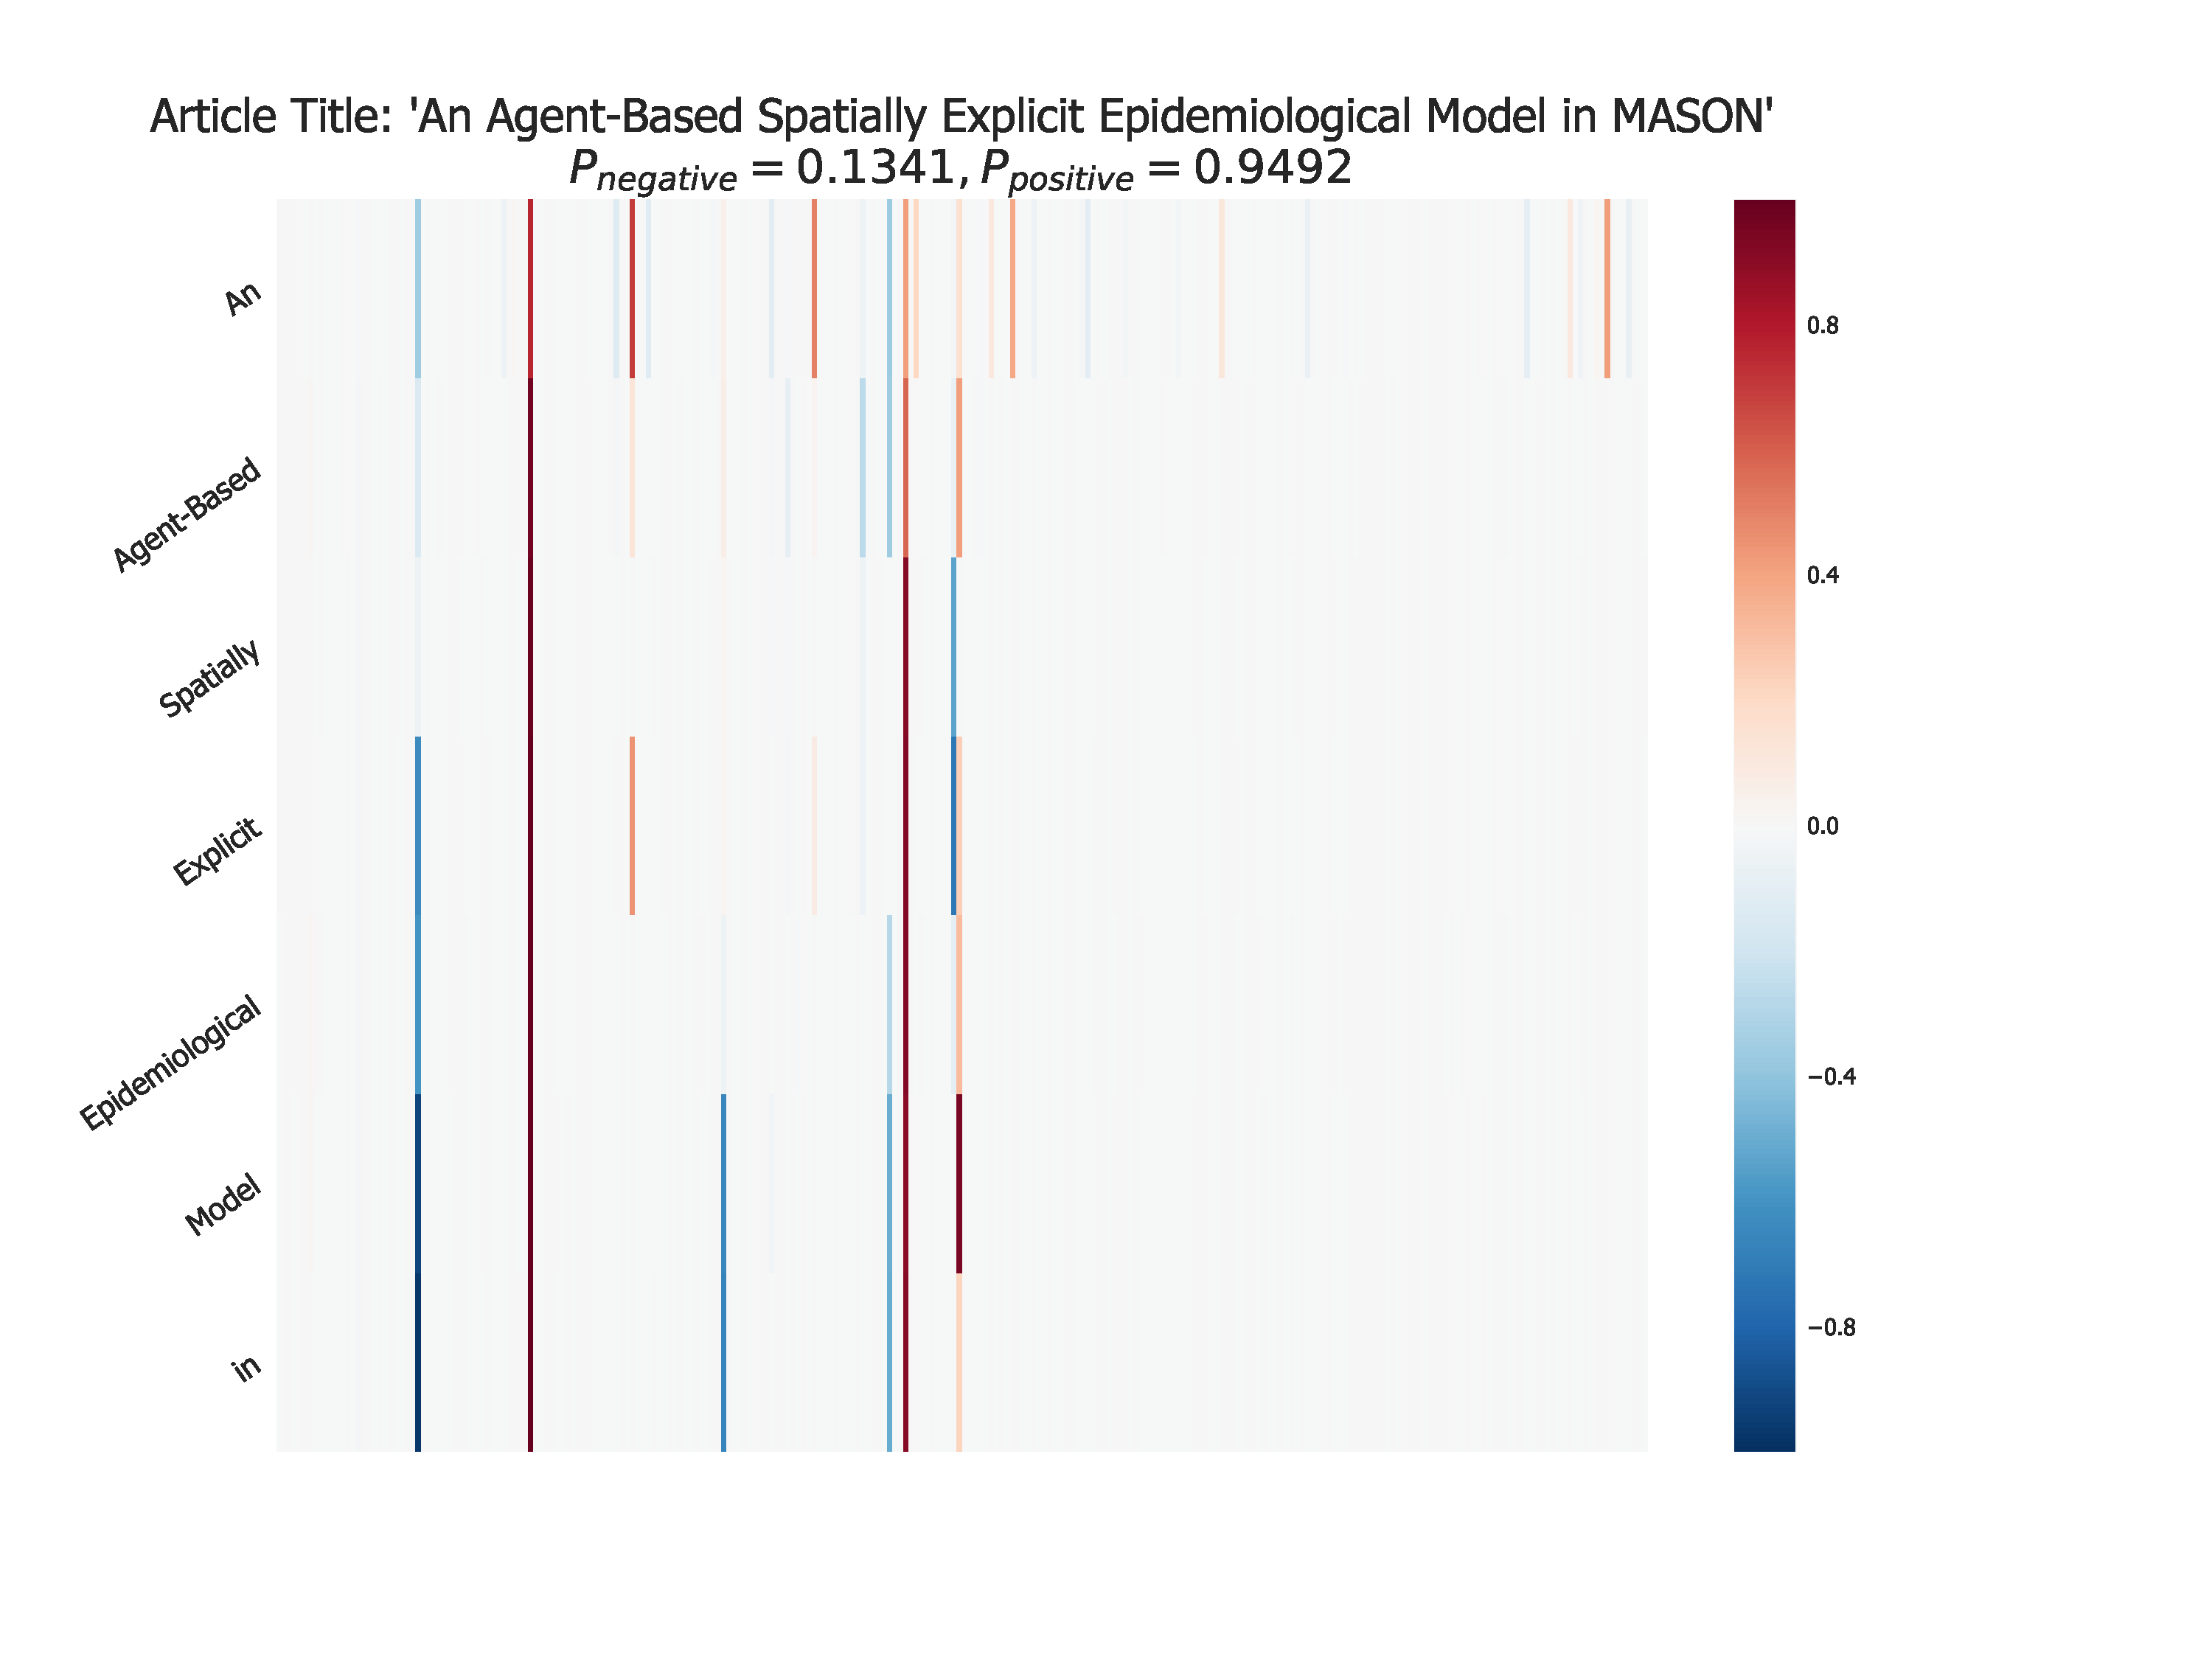
\includegraphics[width=1\textwidth]{activations}
		\end{adjustbox}
		\caption{Example of output activations for a positive example}\label{acts}
	\end{figure}
	
\end{document}